% Design: one key or value tensor of the cache as extents. The rows of the
% prefix are pages of the publisher's file, mapped read-only by every agent;
% the page in which the prefix ends is copied, since it also receives rows of
% the agent. Below, the private extent enlarged: the CPU populates a window of
% rows ahead of the row that the GPU writes, with one call per tensor.
\documentclass[border=2pt]{standalone}
% Shared TikZ style of the STATOR design figures. Teal marks shared,
% immutable state; amber marks what one process writes; violet marks a
% second level of sharing; text is regular weight except the panel titles.
\usepackage{newtxtext}
\usepackage{tikz}
\usetikzlibrary{arrows.meta, positioning, fit, calc, patterns, shapes.geometric, decorations.pathreplacing}

\definecolor{panel}{HTML}{F3F4F6}   % a group of components
\definecolor{gpuc}{HTML}{E4E0F6}    % the GPU
\definecolor{ptc}{HTML}{FAF0DC}     % page tables and the SMMU
\definecolor{modelc}{HTML}{CDEBE6}  % the weights
\definecolor{sharedc}{HTML}{7FCBC1} % shared rows, read-only
\definecolor{tailc}{HTML}{F7B955}   % rows of one process, in use
\definecolor{aheadc}{HTML}{FCE6C2}  % populated ahead, or write-protected
\definecolor{copyc}{HTML}{F4BFCB}   % a copied page
\definecolor{segc}{HTML}{B7A9E8}    % the segment of a second ancestor
\definecolor{faultc}{HTML}{E8736A}  % a private copy made by a fault
\definecolor{actc}{HTML}{FDE9C9}    % an operation of the design
\definecolor{roline}{HTML}{14786F}  % read-only mappings
\definecolor{rwline}{HTML}{C5432F}  % writable mappings and faults

\tikzset{
  layer/.style={draw=black!60, fill=panel, line width=0.5pt},
  sub/.style={draw=black!55, line width=0.4pt},
  comp/.style={draw=black!85, fill=white, line width=0.4pt, align=center,
               font=\scriptsize, inner xsep=3pt, inner ysep=1.5pt, minimum height=0.5cm},
  seg/.style={draw=black!65, line width=0.35pt, inner sep=0pt, align=center,
              font=\scriptsize, minimum height=0.4cm},
  free/.style={seg, pattern=north east lines, pattern color=black!40},
  blk/.style={draw=black!65, line width=0.35pt, minimum width=0.42cm, minimum height=0.36cm,
              inner xsep=2pt, inner ysep=0pt, font=\scriptsize},
  hole/.style={blk, pattern=north east lines, pattern color=black!45},
  tag/.style={font=\scriptsize, inner sep=1pt},
  ttl/.style={font=\bfseries\small},
  lbl/.style={font=\scriptsize},
  note/.style={font=\itshape\scriptsize, inner sep=1pt},
  arr/.style={-{Latex[length=1.6mm]}, line width=0.8pt},
  thin/.style={-{Latex[length=1.3mm]}, line width=0.5pt},
  fat/.style={-{Triangle[length=2.2mm,width=3.4mm]}, line width=2.4pt},
  num/.style={circle, fill=black, text=white, font=\bfseries\scriptsize,
              inner sep=0.6pt, minimum size=0.33cm},
}
% A legend entry: a filled square and its name, at (x,y).
\newcommand{\legendfill}[4]{%
  \draw[black!65, line width=0.35pt, fill=#3] (#1,#2) rectangle ++(0.22,0.2);
  \node[tag, anchor=west] at (#1+0.27,#2+0.1) {#4};}
\newcommand{\legendhatch}[3]{%
  \draw[black!65, line width=0.35pt, pattern=north east lines, pattern color=black!45] (#1,#2) rectangle ++(0.22,0.2);
  \node[tag, anchor=west] at (#1+0.27,#2+0.1) {#3};}
% Legend marks for a legend that is one centred line of text:
%   \node[tag] at (x,y) {\lgdfill{sharedc}\,Shared \quad \lgdhatch\,Unbacked};
\newcommand{\lgdfill}[1]{\tikz[baseline=-0.55ex]{\draw[black!65, line width=0.35pt, fill=#1] (0,-0.1) rectangle (0.22,0.1);}}
\newcommand{\lgdhatch}{\tikz[baseline=-0.55ex]{\draw[black!65, line width=0.35pt, pattern=north east lines, pattern color=black!45] (0,-0.1) rectangle (0.22,0.1);}}

\begin{document}
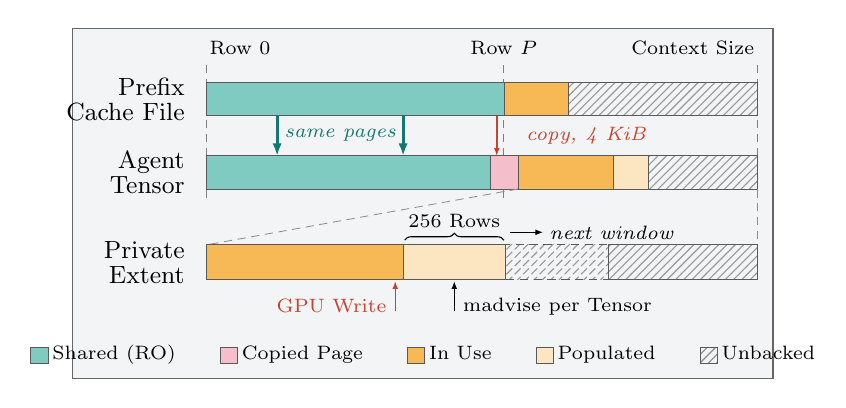
\begin{tikzpicture}[x=1cm, y=1cm, tiny/.style={-{Latex[length=1.0mm]}, line width=0.5pt}]
\draw[layer] (0,0) rectangle (8.9,4.45);

% row axis
\foreach \x in {1.7,5.48,8.7} {
  \draw[black!50, line width=0.3pt, densely dashed] (\x,2.3) -- (\x,3.98);
}
\node[tag, anchor=west] at (1.7,4.2) {Row 0};
\node[tag] at (5.48,4.2) {Row $P$};
\node[tag, anchor=east] at (8.7,4.2) {Context Size};

% the cache file of the publisher: the prefix, then its own rows
\node[font=\small, anchor=east, align=right] at (1.55,3.55) {Prefix\\[-2pt]Cache File};
\node[seg, fill=sharedc, minimum width=3.78cm, minimum height=0.42cm, anchor=west] at (1.7,3.55) {};
\node[seg, fill=tailc, minimum width=0.82cm, minimum height=0.42cm, anchor=west] at (5.48,3.55) {};
\node[free, minimum width=2.4cm, minimum height=0.42cm, anchor=west] at (6.3,3.55) {};

% the tensor of an agent: whole pages of the prefix, the copied page, its rows
\node[font=\small, anchor=east, align=right] at (1.55,2.62) {Agent\\[-2pt]Tensor};
\node[seg, fill=sharedc, minimum width=3.6cm, minimum height=0.42cm, anchor=west] at (1.7,2.62) {};
\node[seg, fill=copyc, minimum width=0.36cm, minimum height=0.42cm, anchor=west] at (5.3,2.62) {};
\node[seg, fill=tailc, minimum width=1.2cm, minimum height=0.42cm, anchor=west] at (5.66,2.62) {};
\node[seg, fill=aheadc, minimum width=0.45cm, minimum height=0.42cm, anchor=west] at (6.86,2.62) {};
\node[free, minimum width=1.39cm, minimum height=0.42cm, anchor=west] at (7.31,2.62) {};

% the same pages, and the page that is copied
\foreach \x in {2.6,4.2} {
  \draw[arr, roline, line width=1.1pt] (\x,3.34) -- (\x,2.83);
}
\node[note, text=roline] at (3.4,3.09) {same pages};
\draw[tiny, rwline] (5.39,3.34) -- (5.39,2.83);
\node[note, text=rwline, anchor=west] at (5.72,3.09) {copy, 4 KiB};

% the private extent, enlarged
\draw[black!45, line width=0.3pt, densely dashed] (5.66,2.41) -- (1.7,1.7);
\draw[black!45, line width=0.3pt, densely dashed] (8.7,2.41) -- (8.7,1.7);
\node[font=\small, anchor=east, align=right] at (1.55,1.48) {Private\\[-2pt]Extent};
\node[seg, fill=tailc, minimum width=2.5cm, minimum height=0.44cm, anchor=west] at (1.7,1.48) {};
\node[seg, fill=aheadc, minimum width=1.3cm, minimum height=0.44cm, anchor=west] at (4.2,1.48) {};
\node[seg, densely dashed, pattern=north east lines, pattern color=black!40, minimum width=1.3cm, minimum height=0.44cm, anchor=west] at (5.5,1.48) {};
\node[free, minimum width=1.9cm, minimum height=0.44cm, anchor=west] at (6.8,1.48) {};
\draw[decorate, decoration={brace, amplitude=2.5pt}] (4.22,1.76) -- (5.48,1.76);
\node[tag] at (4.85,2.0) {256 Rows};
\draw[tiny] (5.56,1.86) -- (5.98,1.86);
\node[note, anchor=west] at (6.02,1.86) {next window};
% the GPU writes behind the window that the CPU populates
\draw[tiny, rwline] (4.1,0.86) -- (4.1,1.24);
\node[tag, text=rwline, anchor=east] at (4.03,0.92) {GPU Write};
\draw[tiny] (4.85,0.86) -- (4.85,1.24);
\node[tag, anchor=west] at (4.92,0.92) {madvise per Tensor};

% legend
\node[tag] at (4.45,0.3) {\lgdfill{sharedc}\,Shared (RO)\qquad\lgdfill{copyc}\,Copied Page\qquad\lgdfill{tailc}\,In Use\qquad\lgdfill{aheadc}\,Populated\qquad\lgdhatch\,Unbacked};
\end{tikzpicture}
\end{document}
